%% --- Trajectory figure (Task 3) ---
%% Yerlesim: Section 8.2 sonrasinda, yer varsa.
%% \input icin: bu dosyayi docs/conference_paper/F3/fig3_trajectory.tex olarak kopyala.
%%
\begin{figure*}[t]
\centering
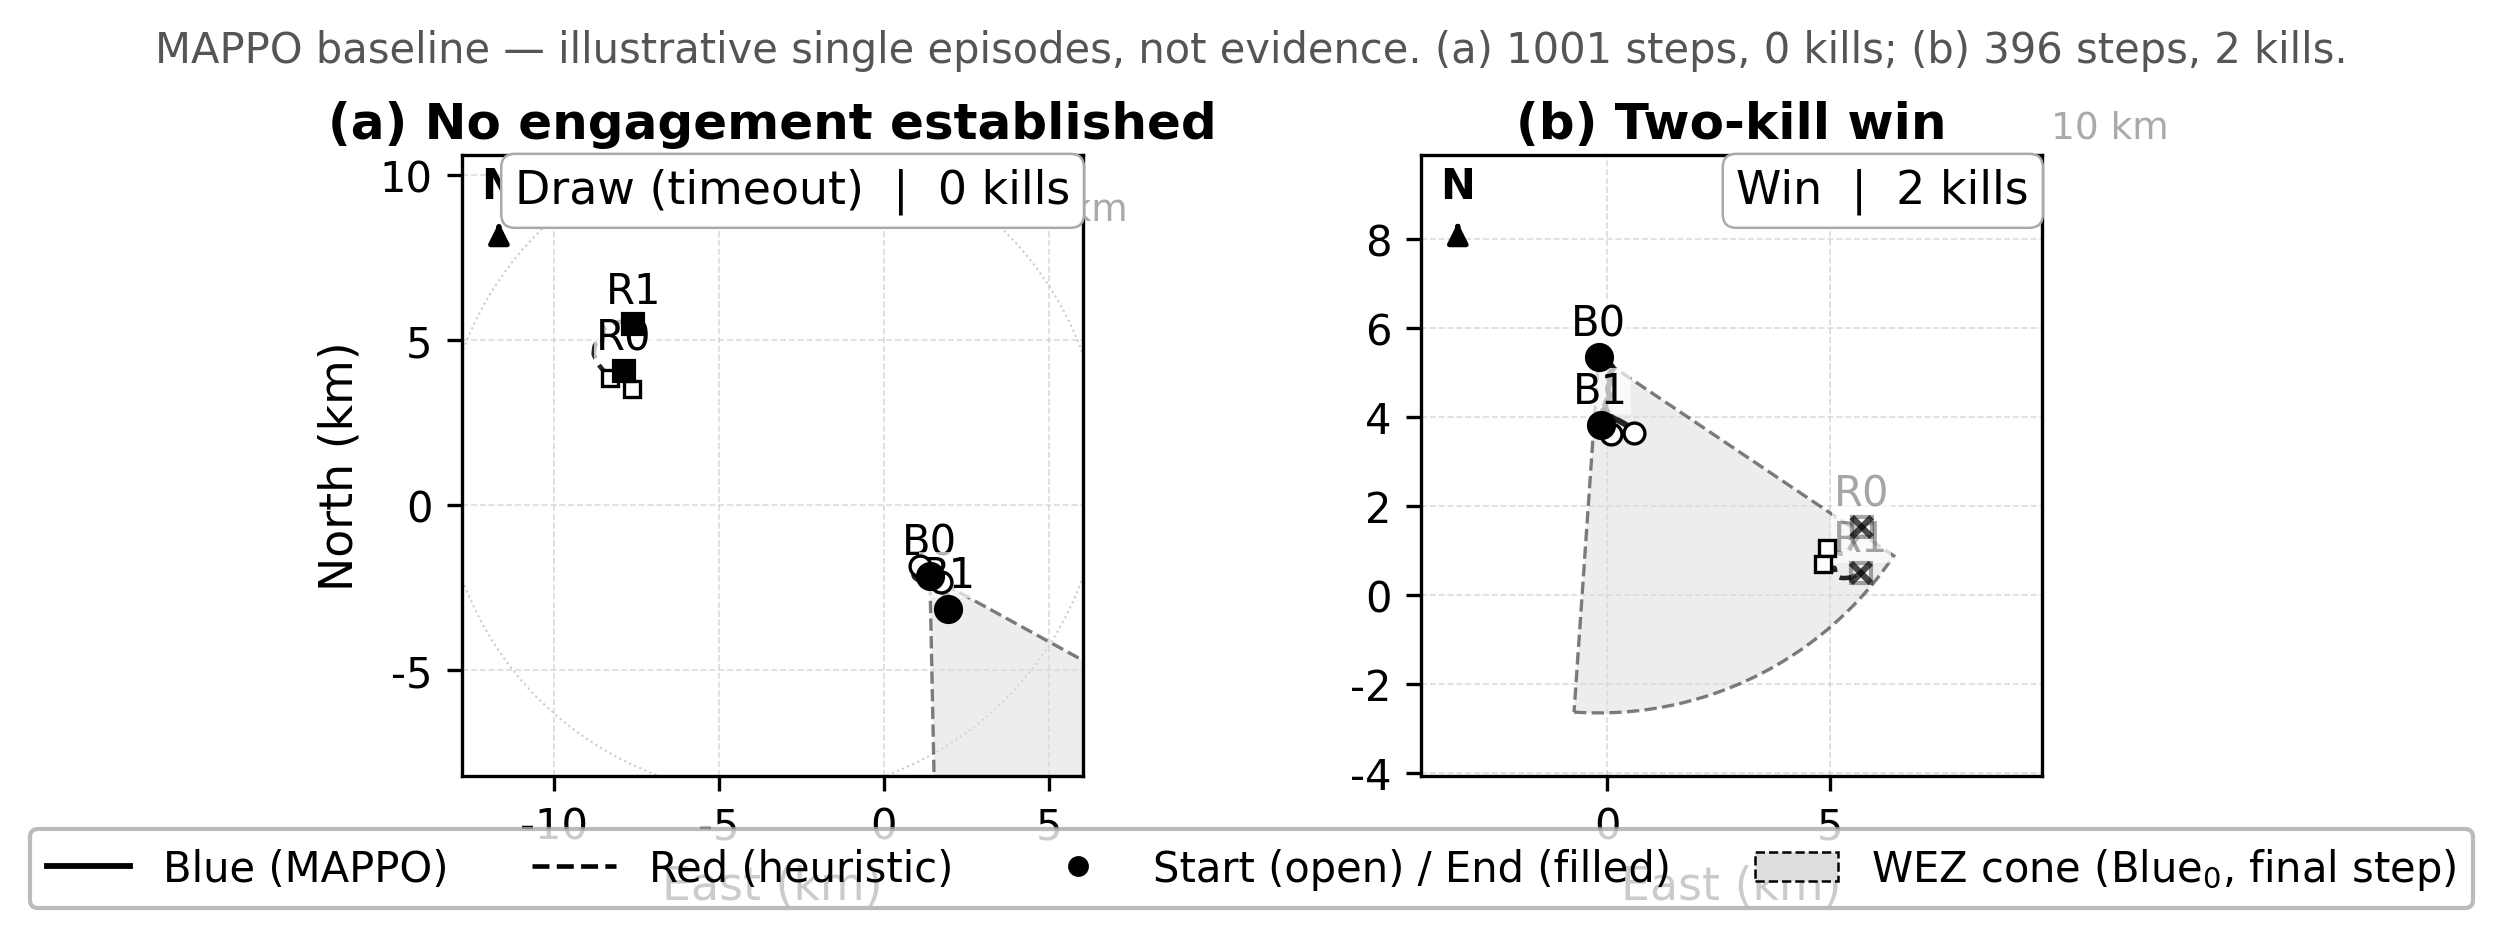
\includegraphics[width=\linewidth]{fig3_trajectory.png}
\caption{%
  Top-down trajectory plots from two illustrative episodes of the MAPPO baseline
  against the heuristic opponent. These are \emph{single hand-picked episodes
  and do not constitute evidence about policy quality}.
  (a)~Zero-kill draw: both Blue agents fail to close within weapon engagement zone
  (WEZ), illustrating the engagement-initiation failure identified in the
  outcome decomposition.
  (b)~Two-kill win: Blue engages and defeats both Red agents within
  396 steps.
  Solid lines: Blue (MAPPO); dashed lines: Red (heuristic).
  Gray wedge: WEZ cone (Blue$_0$, final step only).
  All trajectories are top-down (altitude not shown).%
}
\label{fig:trajectory}
\end{figure*}
